\chapter{Práctico 1 - Parte 2}
\section{Ejercicio 1}

\begin{itemize}
    \item[a)] Ordená los arreglos del ejercicio 4 del práctico anterior utilizando el algoritmo de ordenación por intercalación.
    \item[b)] En el caso del inciso a) del ejercicio 4, dar la secuencia de llamadas al procedimiento merge\_sort\_rec con los valores correspondientes de sus argumentos.
  \end{itemize}

\subsection{Solución (a)}

\begin{figure}[h]
    \centering
    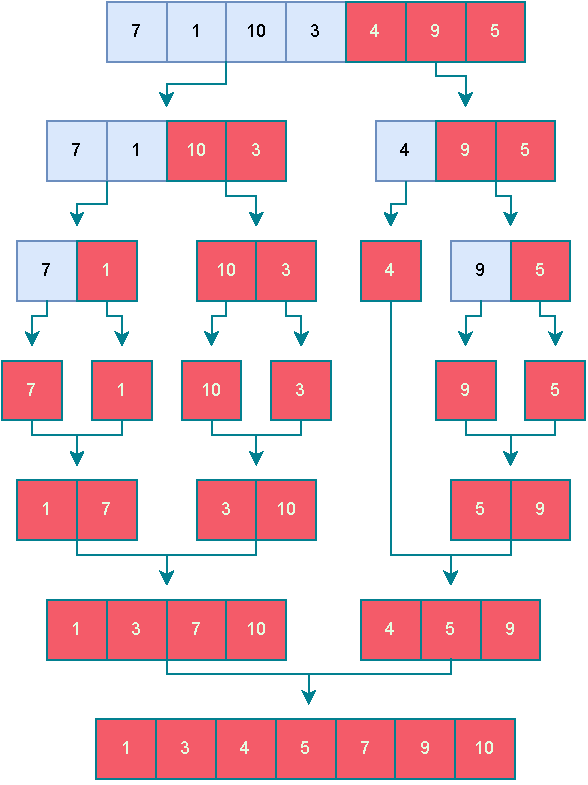
\includegraphics[width=0.6\textwidth]{./estáticos/1a.pdf}
\end{figure}

\begin{tabularx}{\textwidth}{|p{2cm}|X|X|p{2cm}|X|}
    \hline
    \textbf{Iteración} & \textbf{Llamada} & \textbf{Condición rgt > lft} & \textbf{mid} & \textbf{a[lft,rgt]} \\
    \hline
    0 & merge\_sort\_rec(a,1,7) & True & 4 & [7,1,10,3,4,9,5] \\
    1 & merge\_sort\_rec(a,1,4) & True & 2 & [7,1,10,3] \\
    2 & merge\_sort\_rec(a,1,2) & True & 1 & [7,1] \\
    3 & merge\_sort\_rec(a,1,1) & False & - & [7] \\
    4 & merge\_sort\_rec(a,2,2) & False & - & [1] \\
    \hline
    2 & merge(a,1,1,2) & - & 1 & [1,7] \\
    \hline
    2 & merge\_sort\_rec(a,3,4) & True & 3 & [10,3] \\
    3 & merge\_sort\_rec(a,3,3) & False & - & [10] \\
    4 & merge\_sort\_rec(a,4,4) & False & - & [3] \\
    \hline
    2 & merge(a,3,3,4) & - & 3 & [3,10] \\
    \hline
    0 & merge\_sort\_rec(a,5,7) & True & 6 & [4,9,5] \\
    1 & merge\_sort\_rec(a,5,6) & True & 5 & [4,9] \\
    2 & merge\_sort\_rec(a,5,5) & False & - & [4] \\
    3 & merge\_sort\_rec(a,6,6) & False & - & [9] \\
    \hline
    1 & merge(a,5,5,6) & - & 5 & [4,9] \\
    \hline
    1 & merge\_sort\_rec(a,7,7) & False & - & [5] \\
    \hline
    1 & merge(a,1,2,4) & - & 2 & [1,3,7,10] \\
    \hline
    0 & merge(a,5,6,7) & - & 6 & [4,5,9] \\
    \hline
    0 & merge(a,1,4,7) & - & 4 & [1,3,4,5,7,9,10] \\
    \hline
\end{tabularx}

\section{Ejercicio 2}
\begin{itemize}
    \item[a)] Escribí el procedimiento "\texttt{intercalar\_cada}" que recibe un arreglo $a : array[1..2^n] of int$ y un número natural $i : nat$; e intercala el segmento $a[1, 2^i]$ con $a[2^i + 1, 2 * 2^i]$, el segmento $a[2 * 2^i + 1, 3 * 2^i]$ con $a[3 * 2^i + 1, 4 * 2^i]$, etc. Cada uno de dichos segmentos se asumen ordenados. Por ejemplo, si el arreglo contiene los valores $3, 7, 1, 6, 1, 5, 3, 4$ y se lo invoca con con $i = 1$ el algoritmo deberá devolver el arreglo $1, 3, 6, 7, 1, 3, 4, 5$. Si se lo vuelve a invocar con este nuevo arreglo y con $i = 2$, devolverá $1, 1, 3, 3, 4, 5, 6, 7$ que ya está completamente ordenado. El algoritmo asume que cada uno de estos segmentos está ordenado, y puede utilizar el procedimiento de intercalación dado en clase
    \item[b)] Utilizar el algoritmo "\texttt{intercalar\_cada}" para escribir una versión iterativa del algoritmo de ordenación por intercalación. La idea es que en vez de utilizar recursión, invoca al algoritmo del inciso anterior sucesivamente con $i = 0, 1, 2, 3,$ etc.
  \end{itemize}

\subsection{Solución (a)}
Primero para definir el procedimiento, va a recibir un arreglo \texttt{a : array[1..$2^n$] of int} y un número natural $i : nat$:

\begin{codebox}{Estructura}
\begin{pascallike}
proc intercalar_cada(in/out a: array[1..$2^n$] of Int, in i: nat)
...
end proc
\end{pascallike}
\end{codebox}
para poder intercalar el arreglo, se va a tener que llamar a la función \texttt{merge}, que toma un arreglo, y 3 posiciones \texttt{lft}, \texttt{mid}, \texttt{rgt}. Entonces hay que definirlas:

\begin{codebox}{Inicialización de variables}
\begin{pascallike}
proc intercalar_cada(in/out a: array[1..$2^n$] of Int, in i: nat)
    var lft, rgt, mid: nat
    ...
end proc
\end{pascallike}
\end{codebox}
Se deberia agregar una variable natural para recorrer cada segmento del arreglo

\begin{codebox}{Inicialización de variables}
\begin{pascallike}
proc intercalar_cada(in/out a: array[1..$2^n$] of Int, in i: nat)
    var lft, rgt, mid: nat {-Variables para llamar a merge-}
    var k: nat {-Variable para recorrer el arreglo-}
    ...
end proc
\end{pascallike}
\end{codebox}
La idea principal es realizar la intercalación de segmentos del arreglo según el valor proporcionado \texttt{i}, cada segmento tiene un tamaño de $2^i$ elementos. Para ello se debe hacer un ciclo while que calcule cada uno de los índices para llamar a la función de intercalación.

\begin{codebox}{Ciclo while}
\begin{pascallike}
proc intercalar_cada(in/out a: array[1..$2^n$] of Int, in i: nat)
    var lft, rgt, mid: nat {-Variables para llamar a merge-}
    var k: nat {-Variable para recorrer el arreglo-}
    while k $\leq$ $2^n$ do
    lft := ... {-Indice inicial del primer segmento-}
    mid := ... {-Indice final del primer segmento-}
    rgt := ... {-Indice final del segundo segmento-}
    merge(a,lft,mid,rgt) {-Llamada a la funcion para intercalar-}
    k := ...
    do
end proc
\end{pascallike}
\end{codebox}
El índice lft será primero $1$, siguiendo la estructura de los segmentos, deberia tomar el valor de $k * 2^i + 1$, luego el medio es $(j+1) * 2^i$ y el final es $(j+2) * 2^i$.

\begin{codebox}{Procedimiento completo}
\begin{pascallike}
proc intercalar_cada(in/out a: array[1..$2^n$] of Int, in i: nat)
    var lft, rgt, mid: nat {-Variables para llamar a merge-}
    var k: nat {-Variable para recorrer el arreglo-}
    while k $\leq$ $2^n$ do
    lft := k * $2^i$ + 1 {-Indice inicial del primer segmento-}
    mid := (k+1) * $2^i$ {-Indice final del primer segmento-}
    rgt := (k+2) * $2^i$ {-Indice final del segundo segmento-}
    merge(a,lft,mid,rgt) {-Llamada a la funcion para intercalar-}
    k := k+2
    do
end proc
\end{pascallike}
\end{codebox}

\subsection{Solución (b)}
\begin{codebox}{Solución}
\begin{pascallike}
proc intercalar_cada_iter (in/out array[1..$2^n$] of int)
    for i := 0 to n-1 do
    intercalar_cada(a,i)
    od
end proc
\end{pascallike}
\end{codebox}

\section{Ejercicio 3}
\begin{itemize}
\item[a)] Ordená los arreglos del ejercicio 4 del práctico anterior utilizando el algoritmo de ordenación rápida.
\item[b)] En el caso del inciso a), dar la secuencia de llamadas al procedimiento quick\_sort\_rec con los valores correspondientes de sus argumentos.
\end{itemize}

\subsection{Solución (a)}
El arreglo es
\begin{equation*}
  \large
  \begin{array}{|r|r|r|r|r|r|r|}
    \hline \textcolor{red}{7} & \textcolor{red}{1} & \textcolor{red}{10} & \textcolor{red}{3} & \textcolor{red}{4} & \textcolor{red}{9} & \textcolor{red}{5} \\ \hline
  \end{array}
\end{equation*}

El algoritmo QuickSort es un algoritmo de ordenamiento eficiente que utiliza la técnica de "divide y vencerás". Funciona seleccionando un elemento del arreglo como pivote y particionando el arreglo alrededor de ese pivote. Luego, ordena las dos particiones resultantes de forma recursiva.

\begin{enumerate}
    \item Seleccionar un elemento como pivote. Por simplicidad, seleccionaremos el primer elemento del arreglo como pivote, es decir, $7$.
    \item Particionar el arreglo alrededor del pivote:
        \begin{itemize}
            \item Elementos menores que el pivote van a la izquierda.
            \item Elementos mayores que el pivote van a la derecha.
            \item El pivote va en el lugar correcto.
        \end{itemize}
        Después de la partición, el arreglo queda así: $[1, 3, 4, 5, 7, 9, 10]$.
    \item Ordenar recursivamente las particiones izquierda y derecha:
        \begin{enumerate}
            \item Partición izquierda: $[1, 3, 4, 5]$
                \begin{enumerate}
                    \item Seleccionar pivote: $1$
                    \item Particionar: $[1, 3, 4, 5]$ (no se necesita particionar más)
                    \item Ordenar recursivamente las particiones vacías (caso base).
                \end{enumerate}
            \item Partición derecha: $[9, 10]$
                \begin{enumerate}
                    \item Seleccionar pivote: $9$
                    \item Particionar: $[9, 10]$ (no se necesita particionar más)
                    \item Ordenar recursivamente las particiones vacías (caso base).
                \end{enumerate}
        \end{enumerate}
    \item Combinar las particiones ordenadas: $[1, 3, 4, 5, 7, 9, 10]$.
\end{enumerate}

Por lo tanto, el arreglo ordenado final es $[1, 3, 4, 5, 7, 9, 10]$.

\subsection{Solución (b)}

La secuencia de llamadas al procedimiento \texttt{quick\_sort\_rec} con los valores correspondientes de sus argumentos es la siguiente:

\begin{tabularx}{\textwidth}{|X|X|X|X|}
  \hline
  \textbf{Llamada} & \textbf{Condición} & \textbf{Pivote} & \textbf{Arreglo} \\
  \hline
  quick\_sort\_rec(a,1,7) & True & 7 & [7,1,10,3,4,9,5] \\
  quick\_sort\_rec(a,1,4) & True & 7 & [7,1,10,3] \\
  quick\_sort\_rec(a,1,2) & True & 7 & [7,1] \\
  quick\_sort\_rec(a,1,1) & False & 7 & [7] \\
  quick\_sort\_rec(a,2,2) & False & 1 & [1] \\
  quick\_sort\_rec(a,3,4) & True & 7 & [10,3] \\
  quick\_sort\_rec(a,3,3) & False & 10 & [10] \\
  quick\_sort\_rec(a,4,4) & False & 3 & [3] \\
  quick\_sort\_rec(a,5,7) & True & 7 & [4,9,5] \\
  quick\_sort\_rec(a,5,6) & True & 4 & [4,9] \\
  quick\_sort\_rec(a,5,5) & False & 4 & [4] \\
  quick\_sort\_rec(a,6,6) & False & 9 & [9] \\
  quick\_sort\_rec(a,7,7) & False & 5 & [5] \\
  \hline
\end{tabularx}

\section{Ejercicio 4}
Escribí una variante del procedimiento partition que en vez de tomar el primer elemento del segmento \texttt{a[izq, der]} como pivot, elige el valor intermedio entre el primero, el último y el que se encuentra en medio del segmento. Es decir, si el primer valor es 4, el que se encuentra en el medio es 20 y el último es 10, el algoritmos deberá elegir como pivot al último.

\subsection{Solución}
\textbf{Procedimiento \texttt{partition} original:}

\begin{codebox}{Partition}
\begin{pascallike}
proc partition(in/out a: array[1..n] of T, in lft,rgt: nat, out ppiv: nat)
    var i,j: nat
    ppiv:= lft
    i:= lft+1
    j:= rgt
    do i <= j --> if a[i] <= a[ppiv] --> i:= i+1
                    a[j] >= a[ppiv] --> j:= j-1
                    a[i] > a[ppiv] && a[j] < a[ppiv] --> swap(a,i,j)
                fi
    od
    swap(a,ppiv,j)
    ppiv:= j
end proc
\end{pascallike}
\end{codebox}

\textbf{Procedimiento \texttt{partition} modificado:}

\begin{codebox}{Partition modificado}
\begin{pascallike}
proc partition(in/out a: array[1..n] of T, in lft,rgt: nat, out ppiv: nat)
    var i,j: nat
    {-Modificacion al tomar el pivot-}
    if a[lft] <= a[rgt] -->
    if a[lft] <= a[mid] -->
        if a[mid] <= a[rgt] -->
        ppiv := mid
        [] -->
        ppiv := rgt
        fi
        [] -->
        ppiv := lft
        fi
    [] -->
    if a[rgt] <= a[mid] -->
        ppiv := mid
    [] -->
        ppiv := rgt
    fi
    fi
    {--------------------------------}
    i:= lft+1
    j:= rgt
    do i <= j --> if a[i] <= a[ppiv] --> i:= i+1
                    a[j] >= a[ppiv] --> j:= j-1
                    a[i] > a[ppiv] $\wedge$ a[j] < a[ppiv] --> swap(a,i,j)
                fi
    od
    swap(a,ppiv,j)
    ppiv:= j
end proc
\end{pascallike}
\end{codebox}

\section{Ejercicio 5}
Escribí un algoritmo que dado un arreglo \texttt{a : array[1..n] of int} y un número natural $k \leq n$ devuelve el elemento de \texttt{a} que quedaría en la celda \texttt{a[k]} si a estuviera ordenado. Está permitido realizar intercambios en \texttt{a}, pero no ordenarlo totalmente. La idea es explotar el hecho de que el procedimiento partition del quick sort deja al pivot en su lugar correcto.

\subsection{Solución}

\begin{codebox}{Algoritmo}
\begin{pascallike}
fun encontrarElemento(a: array[1..n] of int, k: nat): ret r : int
    var lft, rgt, ppiv: nat

    lft := 1
    rgt := n

    do lft < rgt -->
        partition(a, lft, rgt, ppiv)

        if ppiv = k -->
            r := a[ppiv]
        [] ppiv < k -->
            lft := ppiv + 1
        [] -->
            rgt := ppiv - 1
        fi
    od

    r := a[k]
end proc
\end{pascallike}
\end{codebox}

\section{Ejercicio 6}
El procedimiento \texttt{partition} que se dio en clase separa un fragmento de arreglo principalmente en dos segmentos: menores o iguales al pivot por un lado y mayores o iguales al pivot por el otro. Modificá ese algoritmo para que separe en tres segmentos: los menores al pivot, los iguales al pivot y los mayores al pivot. En vez de devolver solamente la variable \texttt{pivot}, deberá devolver \texttt{pivot izq} y \texttt{pivot} der que informan al algoritmo \texttt{quick\_sort\_rec} las posiciones inicial y final del segmento de repeticiones del \texttt{pivot}. Modificá el algoritmo \texttt{quick\_sort\_rec} para adecuarlo al nuevo procedimiento \texttt{partition}.

\subsection{Solución}

\textbf{Procedimiento \texttt{partition} modificado:}

\begin{codebox}{Partition modificado}
\begin{pascallike}
proc partition(in/out a: array[1..n] of T, in lft, rgt: nat, 
out pivotIzq, pivotDer: nat)
    var i, j, pivotPos: nat
    {-pivotPos rastrea la posicion actual del pivote-}
    pivotPos := lft
    i := lft + 1
    j := rgt

    do i <= j -->
        {-Casos para manejar elementos menores, mayores e iguales al pivote-}
        if a[i] < a[pivotPos] -->
            i := i + 1
        [] a[j] > a[pivotPos] -->
            j := j - 1
        [] a[i] > a[pivotPos] -->
            swap(a, i, j)
        {-Caso para manejar repeticiones del pivote-}
        [] -->
            swap(a, i, pivotPos)
            pivotPos := i
            i := i + 1
            j := j - 1
        fi
    od
    {-pivotIzq es la posicion inicial del segmento de repeticiones del pivote-}
    pivotIzq := lft
    {-pivotDer es la posicion final del segmento de repeticiones del pivote-}
    pivotDer := j
    {-Mover todas las repeticiones del pivote a posiciones contiguas despues de pivotIzq-}
    do j < rgt -->
        swap(a, j + 1, rgt)
        j := j + 1
    od
end proc

proc quick_sort_rec(in/out a: array[1..n] of T, in lft, rgt: nat)
    var pivotIzq, pivotDer: nat

    if lft < rgt -->
        partition(a, lft, rgt, pivotIzq, pivotDer)
        quick_sort_rec(a, lft, pivotIzq - 1)
        quick_sort_rec(a, pivotDer + 1, rgt)
    fi
end proc
\end{pascallike}
\end{codebox}